\documentclass[a3paper,landscape]{article}
\usepackage[provide=*,spanish]{babel}
\usepackage{fontspec}
\setsansfont{Latin Modern Sans}
\renewcommand{\familydefault}{\sfdefault}
\usepackage[margin=10mm]{geometry}
\usepackage{tikz,xcolor,hyperref}
\usetikzlibrary{arrows.meta,positioning}
\pagestyle{empty}
\definecolor{navy}{HTML}{14324C}
\definecolor{teal}{HTML}{008A89}
\definecolor{mint}{HTML}{E4F5F2}
\definecolor{blue}{HTML}{E9F1FA}
\definecolor{gold}{HTML}{FFF2DC}
\definecolor{coral}{HTML}{FCEBE6}
\newcommand{\cardtitle}[1]{{\color{navy}\bfseries\fontsize{18}{21}\selectfont #1}}
\begin{document}
\fontsize{13}{16}\selectfont
\noindent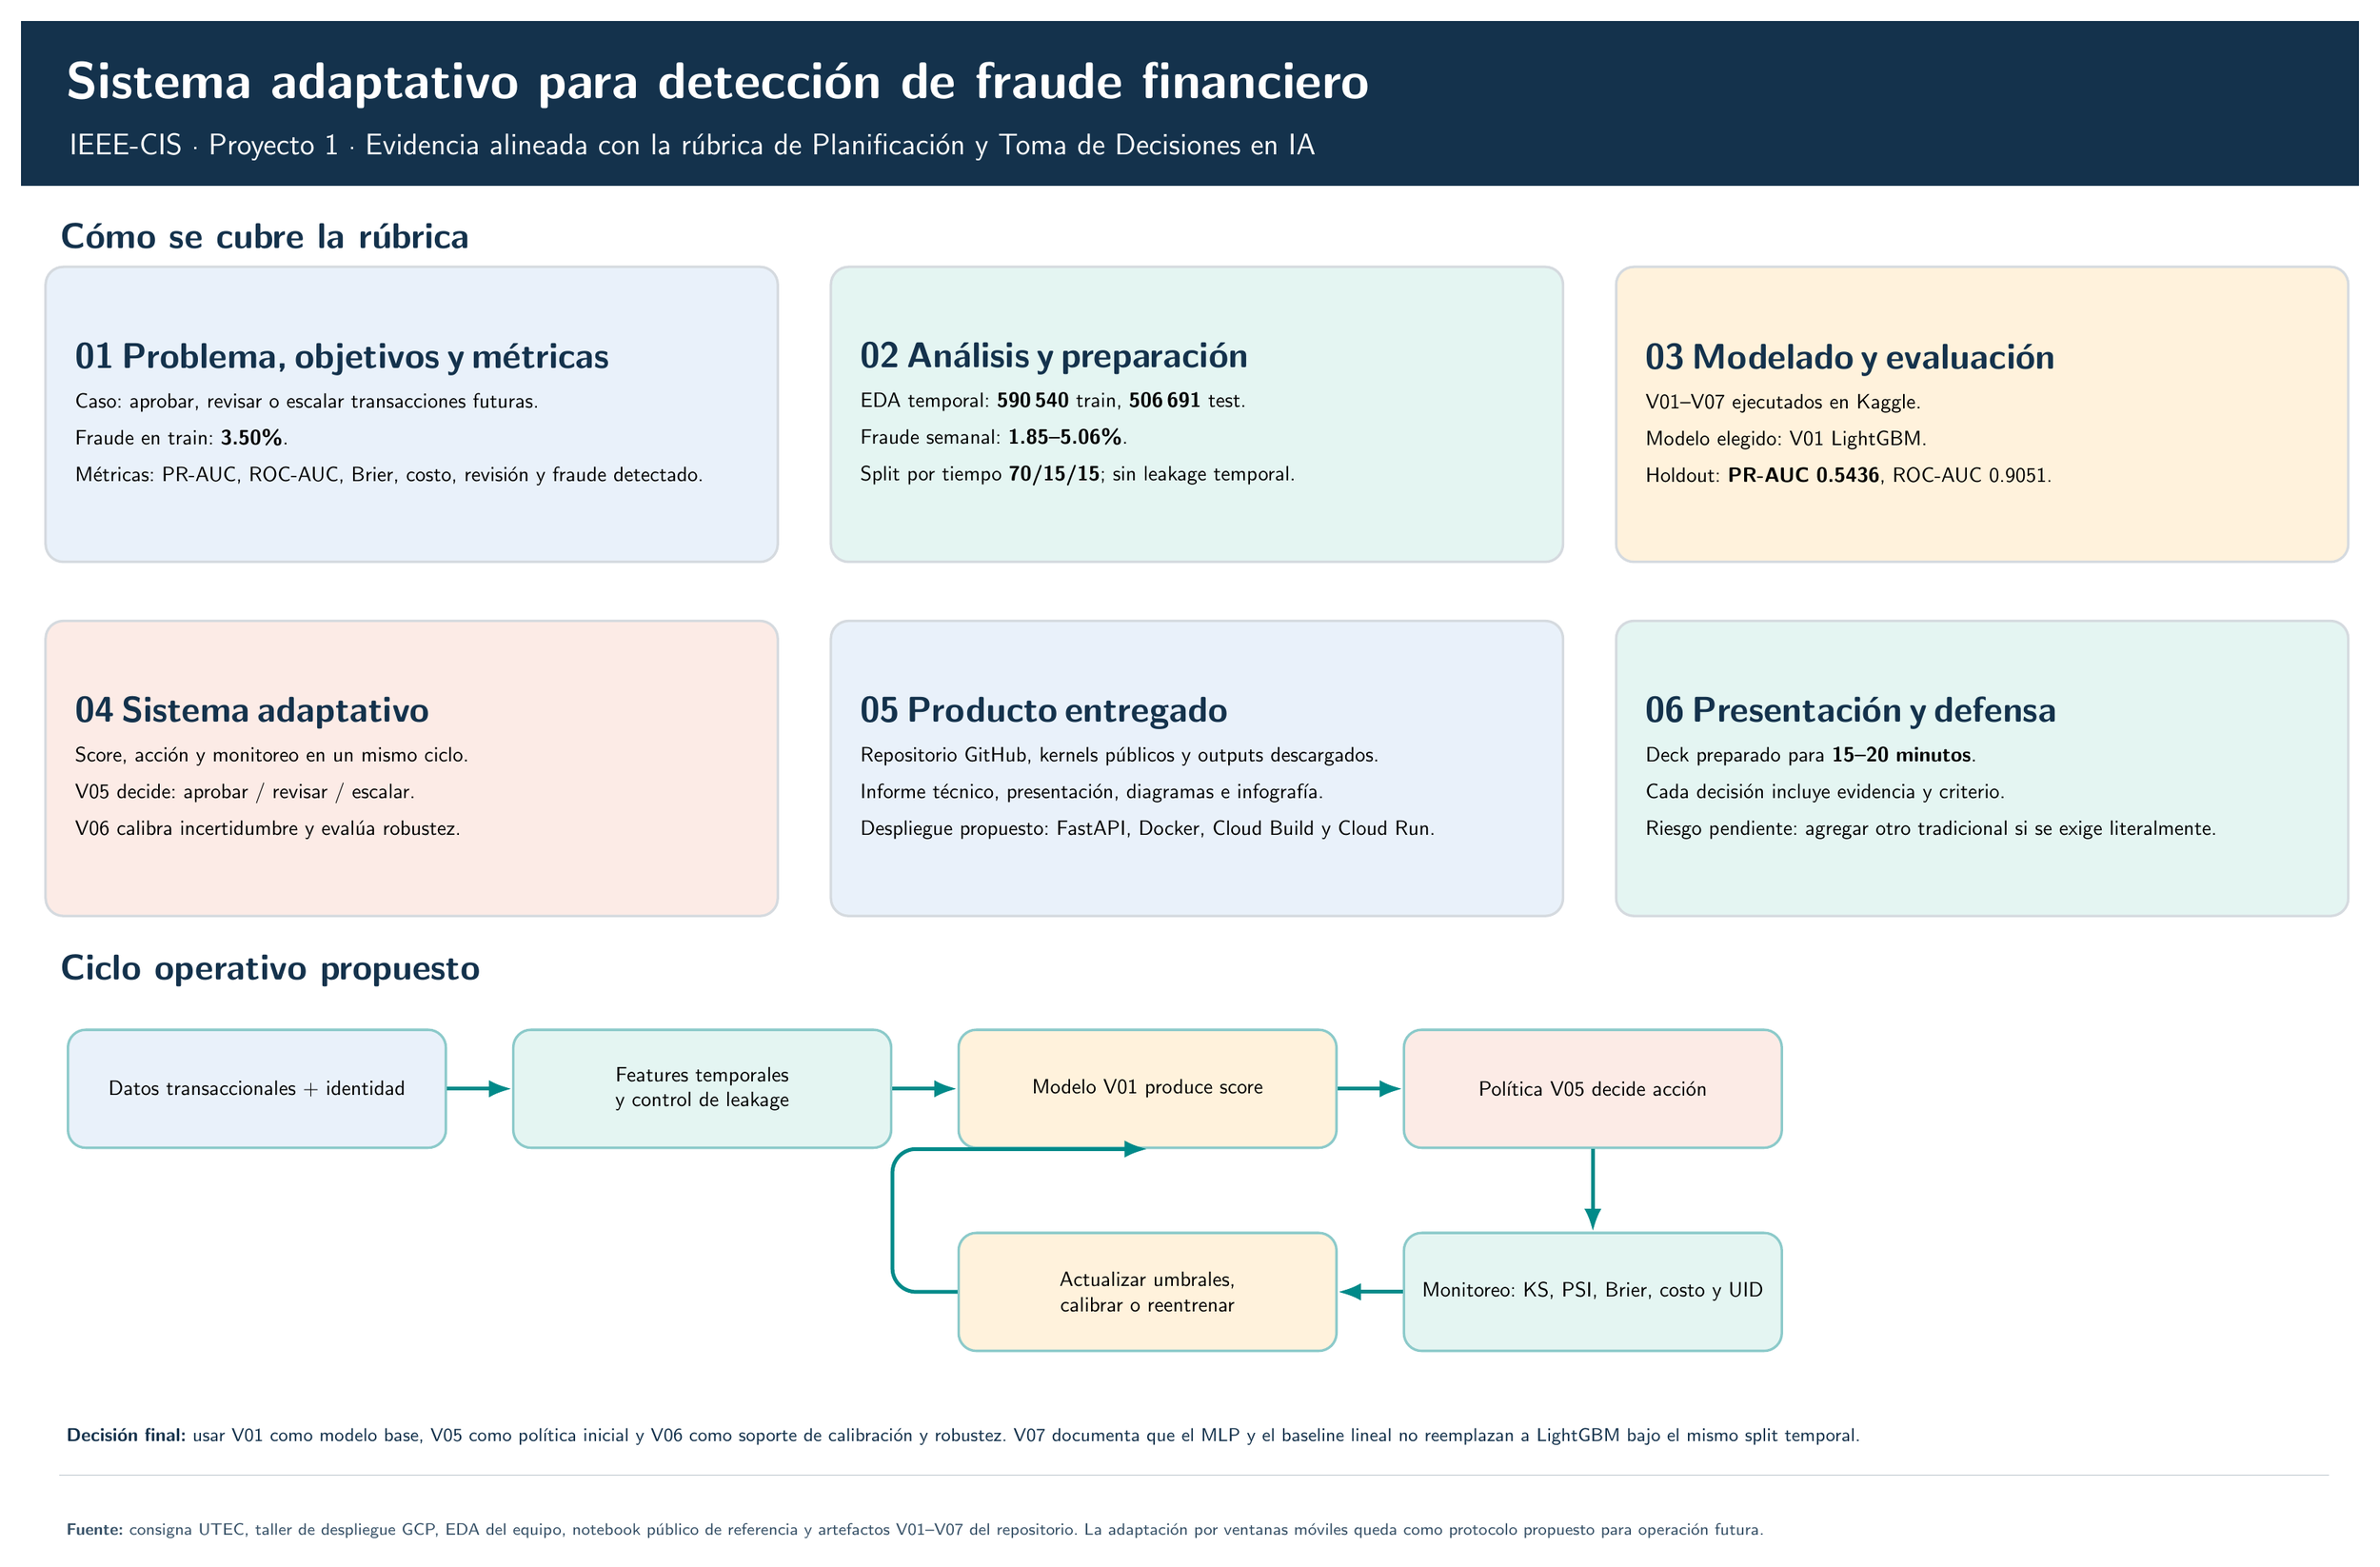
\begin{tikzpicture}[x=1cm,y=1cm,>=Latex,
rubric/.style={draw=navy!18,rounded corners=3mm,very thick,align=left,text width=11.4cm,minimum width=12.1cm,minimum height=5.0cm,inner sep=5mm},
flow/.style={draw=teal!45,rounded corners=3mm,very thick,align=center,text width=5.8cm,minimum width=6.2cm,minimum height=2.0cm,inner sep=3mm},
path/.style={->,line width=1.8pt,teal,rounded corners=4mm}]

\fill[navy] (-.2,24.1) rectangle (39.4,26.9);
\node[anchor=west,text=white,font=\bfseries\fontsize{26}{29}\selectfont] at (.45,25.8){Sistema adaptativo para detección de fraude financiero};
\node[anchor=west,text=white!82,font=\fontsize{13.5}{16}\selectfont] at (.5,24.75){IEEE-CIS · Proyecto 1 · Evidencia alineada con la rúbrica de Planificación y Toma de Decisiones en IA};

\node[anchor=west,text=navy,font=\bfseries\fontsize{18}{21}\selectfont] at (.35,23.25){Cómo se cubre la rúbrica};

\node[rubric,fill=blue,anchor=north west] (r1) at (.2,22.75){\cardtitle{01 Problema, objetivos y métricas}\\[2.5mm]
Caso: aprobar, revisar o escalar transacciones futuras.\\[2mm]
Fraude en train: \textbf{3.50\%}.\\[2mm]
Métricas: PR-AUC, ROC-AUC, Brier, costo, revisión y fraude detectado.};

\node[rubric,fill=mint,anchor=north west] (r2) at (13.5,22.75){\cardtitle{02 Análisis y preparación}\\[2.5mm]
EDA temporal: \textbf{590\,540} train, \textbf{506\,691} test.\\[2mm]
Fraude semanal: \textbf{1.85--5.06\%}.\\[2mm]
Split por tiempo \textbf{70/15/15}; sin leakage temporal.};

\node[rubric,fill=gold,anchor=north west] (r3) at (26.8,22.75){\cardtitle{03 Modelado y evaluación}\\[2.5mm]
V01--V07 ejecutados en Kaggle.\\[2mm]
Modelo elegido: V01 LightGBM.\\[2mm]
Holdout: \textbf{PR-AUC 0.5436}, ROC-AUC 0.9051.};

\node[rubric,fill=coral,anchor=north west] (r4) at (.2,16.75){\cardtitle{04 Sistema adaptativo}\\[2.5mm]
Score, acción y monitoreo en un mismo ciclo.\\[2mm]
V05 decide: aprobar / revisar / escalar.\\[2mm]
V06 calibra incertidumbre y evalúa robustez.};

\node[rubric,fill=blue,anchor=north west] (r5) at (13.5,16.75){\cardtitle{05 Producto entregado}\\[2.5mm]
Repositorio GitHub, kernels públicos y outputs descargados.\\[2mm]
Informe técnico, presentación, diagramas e infografía.\\[2mm]
Despliegue propuesto: FastAPI, Docker, Cloud Build y Cloud Run.};

\node[rubric,fill=mint,anchor=north west] (r6) at (26.8,16.75){\cardtitle{06 Presentación y defensa}\\[2.5mm]
Deck preparado para \textbf{15--20 minutos}.\\[2mm]
Cada decisión incluye evidencia y criterio.\\[2mm]
Riesgo pendiente: agregar otro tradicional si se exige literalmente.};

\node[anchor=west,text=navy,font=\bfseries\fontsize{18}{21}\selectfont] at (.35,10.8){Ciclo operativo propuesto};

\node[flow,fill=blue] (d) at (3.8,8.8){Datos transaccionales + identidad};
\node[flow,fill=mint,right=1.1cm of d] (p) {Features temporales y control de leakage};
\node[flow,fill=gold,right=1.1cm of p] (m) {Modelo V01 produce score};
\node[flow,fill=coral,right=1.1cm of m] (a) {Política V05 decide acción};
\node[flow,fill=mint,below=1.4cm of a] (v) {Monitoreo: KS, PSI, Brier, costo y UID};
\node[flow,fill=gold,left=1.1cm of v] (u) {Actualizar umbrales, calibrar o reentrenar};

\draw[path] (d)--(p);
\draw[path] (p)--(m);
\draw[path] (m)--(a);
\draw[path] (a)--(v);
\draw[path] (v)--(u);
\draw[path] (u.west) -- ++(-1.1,0) |- (m.south);

\node[anchor=west,align=left,text width=37.8cm,font=\small,text=navy] at (.45,2.9){\textbf{Decisión final:} usar V01 como modelo base, V05 como política inicial y V06 como soporte de calibración y robustez. V07 documenta que el MLP y el baseline lineal no reemplazan a LightGBM bajo el mismo split temporal.};
\draw[navy!30] (.45,2.25)--(38.9,2.25);
\node[anchor=west,text width=37.8cm,align=left,font=\footnotesize,text=navy!85] at (.45,1.3){\textbf{Fuente:} consigna UTEC, taller de despliegue GCP, EDA del equipo, notebook público de referencia y artefactos V01--V07 del repositorio. La adaptación por ventanas móviles queda como protocolo propuesto para operación futura.};
\end{tikzpicture}
\end{document}
